\chapter{Perifer interaktion}
\label{PeriferInteratkion}
%
\begin{itemize}
  \item Perifer interaktion - de to yderpunkter
  \item Opmærksomhed (perifer opmærksomhed)
  \item Inddrag figur fra projektforslag (side 118 i bogen eller side 6, der er den røde cirkel der ikke)
  \item Hvorfor er det interesant at designe produkter, som kan reagere på perifer interaktion? (fordele og ulemper) 
  \item Microgestures 
  \item Socialt acceptabelt 
  \item Adfærdsændringer
  \item Casual
\end{itemize}
\noindent
%
Perifer interaktion er ikke nyt. Vi gør det alle sammen, når vi i løbet af vores dagligdag foretager adskillige aktiviteter i vores perifere opmærksomhed, \parencite[s. 1]{PDF:PeripheralInteraction}. Det forudsætter dog at disse perifere interaktioner primært retter sig mod ikke-computer-relateret aktiviteter, såsom at føre en samtale imedens der laves mad. Rettes fokus derimod til \textit{Human-Computer-Interaction}, HCI, så forlanger diverse elektroniske apparater vores centrale opmærksomhed ved at blinke, ringe og vibrere, \parencite[s. 1]{PDF:PeripheralInteraction}. Ifølge \textcite[s. 3]{PDF:PeripheralInteraction} så bevæger interaktionen med elektroniske apparater sig uforudsigeligt mellem den centrale og perifere opmærksomhed, i modsætning til ikke-computer-relateret aktiviteter, som i større grad kan kontrolleres. Grunden til at disse apparater frit kan bevæge sig fra den perifere til den centrale opmærksomhed skyldes, at vi sjælendt har kontrol over hvornår et apparat kræver den centrale opmærksomhed. Så snart et elektronisk apparat befinder sig i den centrale opmærksomhed, så vil ens opmærksomhed midlertidigt fjernes fra den primære opgave, indtil interaktionen med apparatet er afsluttet. Konsekvenserne af at blive forstyrret og skulle rette opmærksomheden væk fra ens primære opgave over til apparatet, er en øget kognitiv belastning samt en større risiko for at begå fejl i den primære opgave, \parencite[ss. 188-189][s. 162]{PDF:PeripheralInteraction, PDF:ComparingInputModalities}. 

Istedet for at forstætte med at designe elektroniske apparater, som kræver den centrale opmærksomhed samt kræver at opmærksomheden flyttes fra den primære opgave over til apparatet, så bør apparaterne derimod designes så de i højere grad bliver en integreret del af vores daglige rutiner, \parencite[s. 239]{PDF:PICharacteristicsAndConsiderations}. Ved at designe apparater ud fra den tilgang så vil det tillade perifer interaktion, fordi det bygger på teori omkring delt-opmærksomhed. Ifølge disse teorier råder mennesket over en bestemt mængde af mentale resourcer, som afhængigt af opgavernes sværhedsgrad, frit kan distribueres mellem opgaverne, \parencite[s. 240]{PDF:PICharacteristicsAndConsiderations}. Derudover tillader delt-opmærksomhed også at flere aktiviteter kan foretages samtidigt, så længe de kun kræve få mentale ressourcer, \parencite[s. 2]{PDF:FacilitatingPIDesignAndEvaluation}. Så istedet for at elektroniske apparater kræver den fulde opmærksomhed, så er det ved perifer interaktion muligt at dele sin opmærksomhed for på den måde at foretage flere aktivitet samtidig. Hvis interaktion med computere og andre elektroniske apparater blev flyttet til det perifere kan det, ifølge \textcite[s. 11]{PDF:TheComputerWeiser}, potentielt være med til at fremme det sociale samvær, som der eksempelvist er på arbejdsmarkedet. Derudover pointerer \textcite[s. 11]{PDF:TheComputerWeiser} at de elektroniske apparater skal tilpasses til den menneskelige hverdag og ikke omvendt. Ligeledes bør designere tage højde for at desto flere elektroniske apparater, der produceres til at fange vores centrale opmærksomhed, desto større er behovet for at en del af interaktionen bliver perifer, \parencite[s. 240]{PDF:PICharacteristicsAndConsiderations}. 

Behovet for at designe elektroniske apparater, som tillader perifer interaktion er ikke nyt. Allerede i halvfemserne blev der af \textcite[s. 3]{PDF:TheComingAgeOfCalmTech} efterspurgt, at såfremt apparaterne skulle være allevegne, så skal de ikke være i vejen. I den forbindelse blev \textit{Calm Technology} skabt. Principperne bag \textit{Calm Technology} er simple; ved at allokere noget af interaktionen i det perifere er det muligt, at håndtere flere informationer ad gangen. Derudover vil denne allokering give en følelse af kontrol, fordi det er muligt selv at kontrollere hvornår noget er i den centrale kontra den perifere opmærksomhed, \parencite[s. 4]{PDF:TheComingAgeOfCalmTech}. Udover perifer interaktion, som blandt andet bygger på \textit{Calm Technology}, tyder det på at der også kan drages nytte af \textit{Casual Interaction}. Ifølge \textcite[ss. 118-119]{PDF:PeripheralInteraction} vedrører \textit{casual interaction} hvor meget kontrol en bruger ønsker at overlevere til et elektronisk apparat.       
%
\begin{figure}[H]
	\centering
	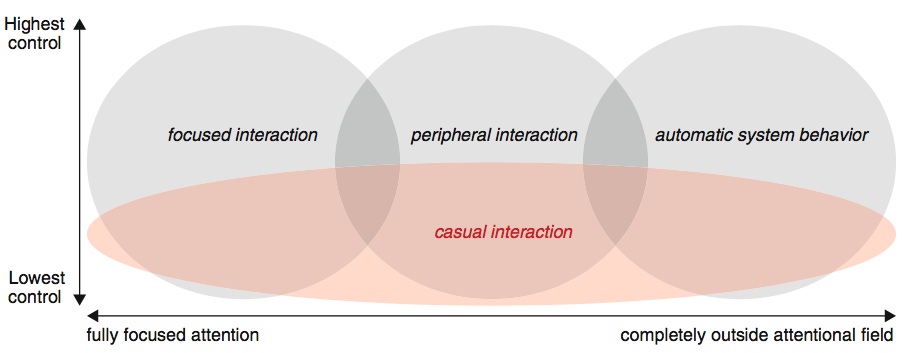
\includegraphics[resolution=300,width=\textwidth]{LevelsOfInteraction}
	\caption{Sammenhæng mellem de tre niveauer af opmærksomhed; central, perifert og automatisk og hvilket niveau af kontrol, der ønskes, \parencite[s. 118]{PDF:PeripheralInteraction}.}
	\label{fig:LevelsOfInteraction}
\end{figure}
\noindent
%


